\documentclass[12pt]{article} % use larger type; default would be 10pt

\usepackage{tikz}
\usetikzlibrary{positioning, automata}
\usetikzlibrary{trees}

\begin{document}

Test graph 2
\\ V1: Position: A speed: 2
\\ V2: Position: C speed: 3
\\
r1 A--B timestep: 0
\\ r2 D--B timestep: 0
\\ r3 B--C timestep: 1
\\r4 A--C timestep: 3 

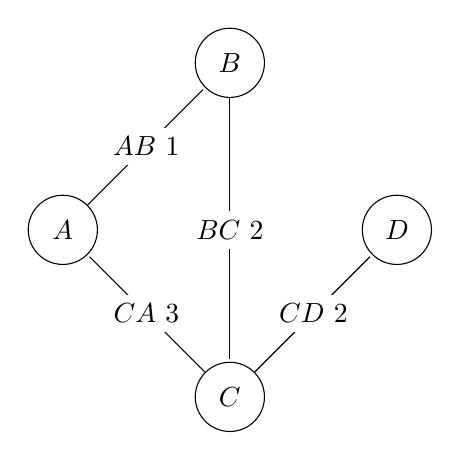
\begin{tikzpicture}[shorten >=1pt,node distance=3cm,on grid,initial/.style    ={}]
  \node[state]          (A)                        {$A$};
  \node[state]          (B) [above right =of A]    {$B$};
  \node[state]          (C) [below right =of A]    {$C$};
  \node[state]          (D) [below right =of B]    {$D$};
\tikzset{mystyle/.style={-}} 
\tikzset{every node/.style={fill=white}} 
\path (A)     edge [mystyle]    node   {$AB\ 1$} (B)
      (C)     edge [mystyle]    node   {$CA\ 3$} (A) 
      (B)     edge [mystyle]    node   {$BC\ 2$} (C)
      (C)     edge [mystyle]    node   {$CD\ 2$} (D);
\end{tikzpicture}

\end{document}